% -*- coding: UTF-8 -*-
% vim: autoindent expandtab tabstop=4 sw=4 sts=4 filetype=tex
% vim: spelllang=de spell
% chktex-file 27 - disable warning about missing include files

\subsection{Ray Marching}
\label{subsec:ray_marching}

~\citeauthor{perlin_hypertexture_1989} schlagen eine Abtastung des
Strahles mit fixen Abständen $\Delta{x_{\mu}}$ vor~\parencite[S.
259]{perlin_hypertexture_1989}:

\begin{gather}
    x = x_{\mu_{0}} + k \cdot \Delta x_{\mu}
\end{gather}

Dabei ist $k = 0,1,2,\dots$ und $\mu_{0} + k \Delta \mu \leq \mu_{1}$.

Auf die parametrische Darstellung eines (Licht-) Strahles,
~\autoref{eq:ray_param_cond}, angewendet, ergibt dies folgende Gleichung:

\begin{gather}
    r(k) = r_{0} + \Delta t \cdot k \cdot r_{d}
\end{gather}

Dabei stellt $\Delta t$ die Grösse der Abstände und $k = 0,1,2,\dots$ die Nummer der
Schritte dar. Wie~\citeauthor{hart_ray_1989} schreiben, bildet das Abtasten des
(Licht-) Strahles mit fixen Abständen die Basis für gewisse Verfahren des
volumetrischen Renderings~\parencite[S. 291]{hart_ray_1989}.

Ein möglicher Algorithmus, wie solch ein Verfahren umgesetzt werden kann,
findet sich in~\autoref{fig:ray_marching}.

\begin{minipage}{\linewidth}
\begin{lstlisting}[language=Python,caption={Eine abstrakte Umsetzung des Ray
        Marchings\protect\footnotemark.},label={fig:ray_marching},captionpos=b,emph={ray_march}]
def ray_march():
    step         = 0
    intersection = 0
    max_steps    = 10

    while step < max_steps:
        intersection = test_intersection(k)

        if intersection <= 0:
            # An intersection has happened
            #   intersection <  0: ray is inside surface
            #   intersection == 0: ray is excatly on surface
            return ray_travel_distance(step)
        # end if

        step = step + 1
    # done while

    # When we reach this step, after max_steps, no intersection
    # has happened, so distance is 0
    return 0
# end ray_march
\end{lstlisting}
\footnotetext{Algorithmus in Pseudocode
    gemäss~\cite{perlin_hypertexture_1989}[S. 259, Abschnitt 3.1]}
\end{minipage}

Dabei ist zu beachten, dass der Abstand der Abtastung eines Strahles
$\Delta{t}$ so gering als möglich sein sollte um eine Menge von Punkten bzw.\ ein
Objekt $A$ --- definiert durch implizite Oberflächen --- möglichst gut
abschätzen zu können. Ist der Abstand zu gross gewählt, so findet ggf.
eine Abtastung weit im Inneren des Objektes statt. Damit geht Präzision
verloren. Es ist weiter möglich, dass der erste eigentliche Punkt gar nicht
abgetastet wird und erst der zweite abgetastete Punkt das Objekt ``erkennt''.

\begin{figure}[H]
    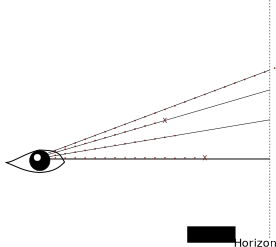
\includegraphics[width=0.8\textwidth]{img/ray_marching_problems.pdf}
    \caption{Illustration des Ray Marching Verfahrens und dessen
        Problematiken.\protect\footnotemark}\label{fig:ray_marching_problems}
\end{figure}
\footnotetext{Eigene Darstellung mittels Inkscape.}

\autoref{fig:ray_marching_problems} veranschaulicht diese
Problematiken. Zu sehen sind vier Primärstrahlen, \textit{e},
\textit{f}, \textit{g} und \textit{h},  sowie zwei Objekte,
\textit{poly1} und \textit{poly2}.

Bei den Strahlen \textit{e} und \textit{f} handelt es sich um
``normale'' Fälle: Der Strahl \textit{e} verfehlt beide Objekte;
das Ray Marching wird also nach Erreichen der maximalen Distanz
\textit{d\textsubscript{max}} abgebrochen.\\
Der Strahl \textit{f} trifft das Objekt \textit{poly1} nach 12
Schritten.

Die Strahlen \textit{g} und \textit{h} sind Spezialfälle: Der Strahl
\textit{g} geht durch das Objekt \textit{poly1}, erfasst dieses wegen
des gewählten fixen Abstandes der Abtastungspunkte ($\Delta{t}$) nicht.
So liegt ein Abtastungspunkt vor dem Objekt und der nächste
Abtastungspunkt bereits in dem Objekt, was zu dem Verfehlen von diesem
führt.

Der Strahl \textit{h} liefert das Objekt \textit{poly2}, obwohl er
eigentlich das Objekt \textit{poly1} liefern müsste. Das getroffene
Objekt \textit{poly2} dürfte so gar nicht zu sehen sein. Dieser Fehler
tritt wiederum aufgrund des gewählten fixen Abstandes der Abtastpunkte
($\Delta{t}$) auf.

\citeauthor{hart_sphere_1994} weist darauf hin, dass Ray Marching durch
den möglichst geringen Abstand zwischen den Abtastungen entsprechend
langsam und paralleles Abtasten praktisch unumgänglich ist~\parencite[S.
528]{hart_sphere_1994}. In der von~\citeauthor{hart_sphere_1994} vorgestellten
Technik des Sphere Tracings ist der Abstand zwischen den Abtastungen
nicht konstant sondern variiert in Abhängigkeit der
Geometrie~\parencite[S. 538 bis 540]{hart_sphere_1994}.

Es wurden verschiedene Methoden entwickelt und untersucht um den
entscheidenden Nachteil des fixen Abstandes der Abtastungspunkte zu
verbessern. So haben zum Beispiel verschiedene Autoren eine Anpassung
des Abstandes mittels Intervall-Arithmetik als Lösung der Problematik
vorgeschlagen~\parencites{caprani_robust_2000}{mitchell_robust_1990}.
